%%%%%%%%%%%%%%%%%%%%%%%%%%%%%%%%%%%%%%%%%
% HW Template
% LaTeX Template
% Version 1.0 (19/10/18)
% Modified by
% Erdem TUNA
% Halil TEMURTAŞ 
% Enes TAŞTAN 
%%%%%%%%%%%%%%%%%%%%%%%%%%%%%%%%%%%%%%%%%
%
%----------------------------------------------------------------------------------------
%	PACKAGES AND OTHER DOCUMENT CONFIGURATIONS
%----------------------------------------------------------------------------------------
\documentclass[a4paper,12pt]{article}
%-----packages------
\usepackage[a4paper, total={6.2in, 8.5in}]{geometry}
\usepackage[english]{babel}
\usepackage[utf8x]{inputenc}
\usepackage{amsmath}
\usepackage{graphicx}
\usepackage[colorinlistoftodos]{todonotes}
\usepackage{gensymb} % this could be problem
\usepackage{float}
\usepackage{fancyref}
\usepackage{subcaption}
\usepackage[toc,page]{appendix} %appendix package
\usepackage{xcolor}
\usepackage{listings}
\usepackage{xspace}
\usepackage{amssymb}
\usepackage{nicefrac}
\usepackage{gensymb}
\usepackage{fancyhdr}
\usepackage{blindtext}  % for dummy text, use \blindtext or \BlindText
\usepackage{lipsum}    % for dummy text, use \lipsum[3-56]
\usepackage[final]{pdfpages}  % pdf include
\usepackage{array} %allows more options in tables
\usepackage{pgfplots,pgf,tikz} %coding plots in latex
\usepackage{capt-of} % allows caption outside the figure environment
\usepackage[export]{adjustbox} %more options for adjusting the images
\usepackage{multicol,multirow,slashbox} % allows tables like table1
%\usepackage[hyperfootnotes=false]{hyperref} % clickable references
\usepackage{epstopdf} % useful when matlab is involved
%\usepackage{placeins} % prevents the text after figure to go above figure with \FloatBarrier 
%\usepackage{listingsutf8,mcode} %import .m or any other code file mcode is for matlab highlighting
\usepackage{enumitem}
\usepackage{hyperref}

%-----end of packages

%-----specifications-----
\definecolor{mGreen}{rgb}{0,0.6,0} % for python
\definecolor{mGray}{rgb}{0.5,0.5,0.5}
\definecolor{mPurple}{rgb}{0.58,0,0.82}
\definecolor{mygreen}{RGB}{28,172,0} % color values Red, Green, Blue for matlab
\definecolor{mylilas}{RGB}{170,55,241}

\setcounter{secnumdepth}{5} % how many sectioning levels to assign numbers to
\setcounter{tocdepth}{5}    % how many sectioning levels to show in ToC

\lstdefinestyle{CStyle}{
	commentstyle=\color{mGreen},
	keywordstyle=\color{magenta},
	numberstyle=\tiny\color{mGray},
	stringstyle=\color{mPurple},
	basicstyle=\footnotesize,
	breakatwhitespace=false,         
	breaklines=true,
	frame=single,
	rulecolor=\color{black!40},                 
	captionpos=b,                    
	keepspaces=true,                 
	numbers=left,                    
	numbersep=5pt,                  
	showspaces=false,                
	showstringspaces=false,
	showtabs=false,                  
	tabsize=2,
	language=C
}

\lstset{language=Matlab,%
	%basicstyle=\color{red},
	breaklines=true,%
	frame=single,
	rulecolor=\color{black!40},
	morekeywords={matlab2tikz},
	keywordstyle=\color{blue},%
	morekeywords=[2]{1}, keywordstyle=[2]{\color{black}},
	identifierstyle=\color{black},%
	stringstyle=\color{mylilas},
	commentstyle=\color{mygreen},%
	showstringspaces=false,%without this there will be a symbol in the places where there is a space
	numbers=left,%
	numberstyle={\tiny \color{black}},% size of the numbers
	numbersep=9pt, % this defines how far the numbers are from the text
	emph=[1]{for,end,break},emphstyle=[1]\color{red}, %some words to emphasise
	%emph=[2]{word1,word2}, emphstyle=[2]{style},    
}


\tikzset{
	desicion/.style={
		diamond,
		draw,
		text width=4em,
		text badly centered,
		inner sep=0pt
	},
	block/.style={
		rectangle,
		draw,
		text width=10em,
		text centered,
		rounded corners
	},
	cloud/.style={
		draw,
		ellipse,
		minimum height=2em
	},
	descr/.style={
		fill=white,
		inner sep=2.5pt
	},
	connector/.style={
		-latex,
		font=\scriptsize
	},
	rectangle connector/.style={
		connector,
		to path={(\tikztostart) -- ++(#1,0pt) \tikztonodes |- (\tikztotarget) },
		pos=0.5
	},
	rectangle connector/.default=-2cm,
	straight connector/.style={
		connector,
		to path=--(\tikztotarget) \tikztonodes
	}
}

\tikzset{
	desicion/.style={
		diamond,
		draw,
		text width=4em,
		text badly centered,
		inner sep=0pt
	},
	block/.style={
		rectangle,
		draw,
		text width=10em,
		text centered,
		rounded corners
	},
	cloud/.style={
		draw,
		ellipse,
		minimum height=2em
	},
	descr/.style={
		fill=white,
		inner sep=2.5pt
	},
	connector/.style={
		-latex,
		font=\scriptsize
	},
	rectangle connector/.style={
		connector,
		to path={(\tikztostart) -- ++(#1,0pt) \tikztonodes |- (\tikztotarget) },
		pos=0.5
	},
	rectangle connector/.default=-2cm,
	straight connector/.style={
		connector,
		to path=--(\tikztotarget) \tikztonodes
	}
}
%-----end of specifications-----


%----commands----
\newcommand\nd{\textsuperscript{nd}\xspace}
\newcommand\rd{\textsuperscript{rd}\xspace}
\newcommand\nth{\textsuperscript{th}\xspace} %\th is taken already
\newcommand{\specialcell}[2][c]{ \begin{tabular}[#1]{@{}c@{}}#2\end{tabular}} % for too long table lines

\newcommand{\blankpage}{
	\- \\[9cm]	
	{ \centering \textit{This page intentionally left blank.} \par }
	\- \\[9cm]
}% For Blank Page

\makeatletter
\renewcommand\paragraph{\@startsection{paragraph}{4}{\z@}%
	{-2.5ex\@plus -1ex \@minus -.25ex}%
	{1.25ex \@plus .25ex}%
	{\normalfont\normalsize\bfseries}}
\makeatother
%-----end of commands-----

\pagestyle{fancy}
\fancyhead[LO,LE]{Halil TEMURTAŞ / 2094522 }
\fancyhead[RO,RE]{December 3, 2018}
\fancyfoot[RO,RE]{
\includegraphics[width=2.7cm]{images/eelogo}}

\begin{document}
\begin{center}
	\textbf{\large EE407 Process Control \\[0.2cm] Experiment 5} \\
\end{center}

\section{\large Mathematical Modelling}
	\begin{enumerate}
		\item A first order transfer function can approximate the temperature of the chamber at the $n^{th}$ sensor for the purpose of designing a temperature controller.
		
			$$ T_n(s)=\frac{K_n}{\tau_n s+1}V_h(s)$$
			
			where $K_n$ is the steady-state gain and $\tau_n$ is the time constant of the $n^{th}$ sensor.
	\end{enumerate}
	
\section{\large Bump Test Identification}
	\begin{enumerate}[resume]
		\item -
	\end{enumerate}
	
\section{\large Time Response Characteristics of 2\nd Order Systems}
	\begin{enumerate}[resume]
		\item The output of the given system at \textit{Figure~\ref{fig:3}} can be written in Laplace domain as
			$$  Y(s) =\frac{C(s)P(s)}{1+C(s)P(s)}R(s)  $$
			\begin{figure}[H]
				\center
				\setlength{\unitlength}{\textwidth} 
				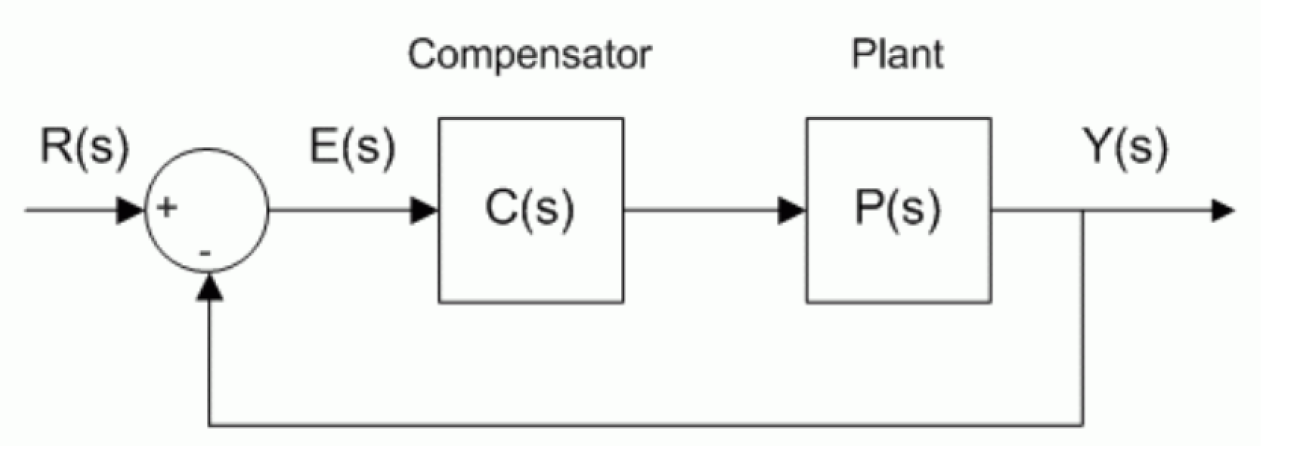
\includegraphics[width=0.7\unitlength]{images/3}
				\caption{\label{fig:3} Block diagram of a negative unit feedback close loop system }
			\end{figure}
		
		\item Error transfer function for \textit{Figure~\ref{fig:3}} can found as follows;
		
			$$ E(s)=R(s)_Y(s)=R(s)\left[ 1 -\frac{C(s)P(s)}{1+C(s)P(s)}\right]$$
			$$ \boxed{ E(s) =\frac{1}{1+C(s)P(s)}R(s) }$$
			
		\item With $C(s)=K_p$, $P(s)=\cfrac{K}{\tau s +1}$, by using the final-value theorem steady state error can be found as follows;
			
			$$ e_{ss} = \lim_{t \to \infty}e(t)=\lim_{s \to 0} sE(s)=\lim_{s \to 0} \cfrac{sR(s)}{1+K_p\ \cfrac{K}{\tau s +1}}$$
			
			With $R(s)=\cfrac{R_0}{s}$
			
			$$ e_{ss} = \cfrac{R_0}{1+K_p\ \lim_{s \to 0}\left( \cfrac{K}{\tau s +1} \right) }$$
			$$\boxed{ e_{ss} =\frac{R_0}{1+K K_p} }$$
			
			
		\item Investigating the steady state error and open loop transfer function, it can be concluded that the system is a Type 0 system. The table at \textit{Table~\ref{tab:6}}\footnote{ \href{http://www.cs.mun.ca/av/old/teaching/cs/notes/steady_printout.pdf}{Memorial University of Newfoundland / Control Systems I / Unit 6: Steady-State Error } } can be examined for more understanding. 
			\begin{table}[H]
				\center
				\setlength{\unitlength}{\textwidth} 
				\caption{\label{tab:6} Steady-State Error Table } 
				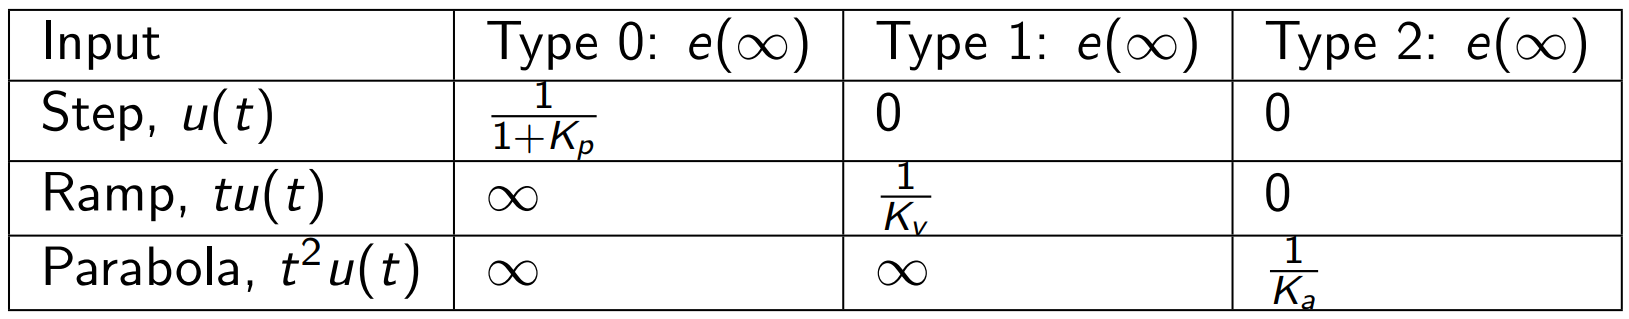
\includegraphics[width=1.0\unitlength]{images/6}
			\end{table}		
		
		\item The closed-loop transfer function can be casted into the standard form given by
			
			$$ G(s)=\frac{Y(s)}{R(s)}=\frac{w_n^2}{s^2+2\xi w_n s + w_n^2} $$
			
			where $w_n$ is the natural frequency and $\xi$ is the damping ratio.
		
		\newpage	
			
		\item 	
			$$\boxed{ \%OS=\frac{y_{peak}-y{ss}}{y_{ss}} = 100\ e^{-\left(\cfrac{\xi \pi}{\sqrt{1- \xi^2}}	\right)} }$$
			$$\boxed{ t_{peak}=\frac{\pi}{w_n \sqrt{1- \xi^2}}=\frac{\pi}{w_d}	}$$
		 
	\end{enumerate}
	
	
\section{\large Performance Requirements for the Heat Flow Experiment}
	\begin{enumerate}[resume]
		\item In this experiment, time-domain performance requirements are specied as follows.
		$$e_{ss}=0\ ,\ t_p=15\ secs\ ,\ PO(\%)=15.0$$
	\end{enumerate}
	
	
\section{\large Temperature Control}
	\subsection{On-Off Control}
	\begin{enumerate}[resume]
		\item -
		\item -
	\end{enumerate}
	
\section{\large Proportional-Integral Control}
	\begin{enumerate}[resume]
		\item -
		\item 
			$$ G(s)=\frac{T(s)}{T_d(s)}$$
			$$ \left[K_p(T_d(s)b_{sp}-T(s))+K_I\left(\frac{T_d(s)_T(s)}{s}\right) \right]\frac{K}{\tau s+1} = T(s)$$ 
			$$ T_d(s)\left[K_p b_{sp}+\frac{K_I}{s} \right]\frac{K}{\tau s+1}=T(s) \left[ 1+\frac{K}{\tau s+1}\left(  K_p+\frac{K_I}{s} \right)	\right] $$
			$$ G(s)=\cfrac{\left[K_p b_{sp}+\cfrac{K_I}{s} \right]\cfrac{K}{\tau s+1}}{1+\cfrac{K}{\tau s+1}\left(  K_p+\cfrac{K_I}{s} \right)}=\cfrac{K\left[K_p b_{sp}+\cfrac{K_I}{s} \right]}{(\tau s +1 )+K\left(  K_p+\cfrac{K_I}{s} \right)}$$
			$$ G(s)=\frac{K K_p b_{sp}s + K K_I}{\tau s^2 +(1+K K_p)s+K K_I}$$
			
			$$ \boxed{ G(s) = \cfrac{ \cfrac{K K_p b_{sp}}{\tau}s + \cfrac{K K_I}{\tau}}{s^2 +\cfrac{1+K K_p}{\tau}s+\cfrac{K K_I}{\tau}} 	}$$
			
		\item
			$$ \boxed{ G(s) \approx  \cfrac{  \cfrac{K K_I}{\tau}}{s^2 +\cfrac{1+K K_p}{\tau}s+\cfrac{K K_I}{\tau}}	}$$ 
			
			$$ G(s)=\frac{w_n^2}{s^2+2\xi w_n s + w_n^2} $$
			with 
			$$\boxed{ w_n = \sqrt{\cfrac{K K_I}{\tau}} }\ \ ,\ \ \boxed{\xi=\cfrac{1+K K_p}{2\tau w_n}	}$$
			Thus,
			$$ \boxed{ K_I = \cfrac{w_n^2 \tau}{K}}\ \ ,\ \ \boxed{K_p=\frac{2 \xi w_n \tau -1}{K}	} $$
		\item
			$$\boxed{ \xi = \cfrac{-ln(\cfrac{\%OS }{100})}{\sqrt{\pi^2+ln^2( \cfrac{\%OS }{100})}} }$$
			
			$$\boxed{ w_n = \cfrac{\pi}{t_p\sqrt{1-\xi^2}} }$$
		\item To meet the requirements at step 9
			$$e_{ss}=0\ ,\ t_p=15\ secs\ ,\ PO(\%)=15.0$$
			
			$$\boxed{ \xi = \cfrac{ -ln(0.15 )}{\sqrt{\pi^2+ln^2(0.15) }}=0.589} $$
			
			$$\boxed{ w_n = \cfrac{\pi}{t_p\sqrt{1-{(0.589)}^2}}=0.355 }$$
			
		\item With $K=0.8$ and $\tau=50$
			$$ \boxed{ K_I = \cfrac{w_n^2 \tau}{K}=\cfrac{{(0.355)}^2 50}{0.8}=7.8765 }$$
			
			$$ \boxed{K_p=\frac{2 \xi w_n \tau -1}{K}=\frac{2 (0.589) (0.355) 50 -1}{0.8}=24.8868	} $$
		\item
			$$ \frac{E(s)}{R(s)}=\frac{1}{1+G_{ol}(s)}=\frac{1}{1+G_{PI}G(s)}$$
			$$ \frac{E(s)}{R(s)}=\cfrac{1}{1+\left(G_p+\cfrac{G_I}{s}\right)\left( \cfrac{K}{\tau s+1}\right)}$$
			with given $K$ and $\tau$
			$$ \frac{E(s)}{R(s)}=\frac{50s^2+s}{50s^2+[1+0.8K_p]s+0.8K_I}$$
		\item 
			$$ e_{ss}=\lim_{s \to 0}sE(s)=\lim_{s \to 0} sR(s)\frac{50s^2+s}{50s^2+[1+0.8K_p]s+0.8K_I}$$
			Using L'Hospital Rule, the limit can be evaluated as follows
			$$ e_{ss}=\lim_{s \to 0} \frac{50s^2+s}{50s^2+[1+0.8K_p]s+0.8K_I}=\lim_{s \to 0}\frac{100s+1}{100s+1+0.8K_p}$$	
			$$\boxed{ e_{ss}=\lim_{s \to 0}\frac{100}{100}=1 }$$
			
			
	
		
	\end{enumerate}
	\subsection{Anti-Windup}
		\begin{enumerate}[resume]
			\item -
			\item -
			\item -
		\end{enumerate}

	
%\begin{appendices}
%\section{Source Code for Matlab Part}\label{appendix}
	%%	\lstinputlisting[language=Matlab,firstline=33, lastline=34]{q13.m} \-\\[1cm]		
%\lstinputlisting[language=Matlab]{EXP1.m} 
%\end{appendices}

\end{document}

\end{document}

%----samples------
%\begin{itemize}
%\item Item
%\item Item
%\end{itemize}

%\begin{figure}[H]
%\center
%\setlength{\unitlength}{\textwidth} 
%\includegraphics[width=0.7\unitlength]{images/logo1}
%\caption{\label{fig:logo}Logo }
%\end{figure}

%\begin{figure}[H]
%	\setlength{\unitlength}{\textwidth} 
%	\centering
%	\begin{subfigure}{.5\textwidth}
%  		\centering
%  		\includegraphics[width=0.48\unitlength]{images/logo1}
%  		\caption{\label{fig:logo1}Logo1 }
%	\end{subfigure}%
%	\begin{subfigure}{.5\textwidth}
%  		\centering
%		\includegraphics[width=0.48\unitlength]{images/logo2}
%  		\caption{\label{fig:logo2}Logo2}
%	\end{subfigure}
%\caption{\label{fig:calisandegree} Small Logos   }
%\end{figure}
	
%\begin{table}[H]
%  \centering
% 
%    \begin{tabular}{c|c|c}
%       $$A$$ & $$B$$ & $$C$$ \\ \hline
%       1 & 2 & 3  \\ \hline
%       2 & 3 & 4  \\ \hline
%       3 & 4 & 5  \\ \hline
%       4 & 5 & 6  
%      
%  \end{tabular}
%  \caption{table}
%  \label{tab:table}
%\end{table}
	
%\begin{table}[H]
%  \centering
% 
%    \begin{tabular}{c|c|c}
%       \backslashbox{$A$}{$a$} & $$\specialcell{ Average deviation \\ after subtracting out the  \\ frequency error }$$ & $$C$$ \\ \hline
%       \multirow{2}{*}{1} & 2 & 3  \\ \cline{2-3}
%        & 3 & 4  \\ \hline
%       3 & \multicolumn{2}{c}{4}  \\ \hline
%       4 & 5 & 6  
%      
%  \end{tabular}
%  \caption{table}
%  \label{tab:table}
%\end{table}
%-----end of samples-----